\documentclass[12pt]{article}
\usepackage[utf8]{inputenc}

\usepackage{enumitem}
\usepackage[margin=2cm]{geometry}

\usepackage{amsmath, amsfonts, amssymb}
\usepackage{graphicx}
\usepackage{tikz}
\usepackage{pgfplots}
\usepackage{multicol}

\usepackage{comment}
\usepackage{url}
\usepackage{calc}
\usepackage{subcaption}
\usepackage{circledsteps}
\usepackage{wrapfig}
\usepackage{array}

\setlength\parindent{0pt}

\usepackage{fancyhdr}
\pagestyle{fancy}
\fancyhf{}
\renewcommand{\headrulewidth}{2pt}
\renewcommand{\footrulewidth}{0pt}
\rfoot{\thepage}
\lhead{\textsc{Math} 244}
\chead{\textsc{Homework 11}}
\rhead{Fall 2023}

\pgfplotsset{compat=1.16}

% MATH commands
\newcommand{\ga}{\left\langle}
\newcommand{\da}{\right\rangle}
\newcommand{\oa}{\left\lbrace}
\newcommand{\fa}{\right\rbrace}
\newcommand{\oc}{\left[}
\newcommand{\fc}{\right]}
\newcommand{\op}{\left(}
\newcommand{\fp}{\right)}

\newcommand{\bi}{\mathbf{i}}
\newcommand{\bj}{\mathbf{j}}
\newcommand{\bk}{\mathbf{k}}
\newcommand{\bF}{\mathbf{F}}

\newcommand{\ra}{\rightarrow}
\newcommand{\Ra}{\Rightarrow}

\newcommand{\sech}{\mathrm{sech}\,}
\newcommand{\csch}{\mathrm{csch}\,}
\newcommand{\curl}{\mathrm{curl}\,}
\newcommand{\dive}{\mathrm{div}\,}

\newcommand{\ve}{\varepsilon}
\newcommand{\spc}{\vspace*{0.5cm}}

\DeclareMathOperator{\Ran}{Ran}
\DeclareMathOperator{\Dom}{Dom}

\newcommand{\exo}[3]{\noindent\textcolor{red}{\fbox{\textbf{Section {#1}, Problem {#2}}}\hrulefill   \textbf{({#3} Pts})}\vspace*{10pt}}

\begin{document}
\thispagestyle{empty}
	\noindent \hrulefill \newline
	MATH-244 \hfill Pierre-Olivier Paris{\'e}\newline
	Homework 11 Solutions \hfill Fall 2023\newline \vspace*{-0.7cm}
	
	\noindent\hrulefill
	
	\spc

	\exo{16.7}{6}{5}
	\\ 
	We have
		\begin{align*}
		\vec{r}_u &= \left\langle \cos v , \sin v , 1 \right\rangle \\ 
		\vec{r}_v &= \left\langle -u \sin v , u \cos v , 0 \right\rangle.
		\end{align*}
	Therefore
		\[
			\vec{r}_u \times \vec{r}_v = \left\langle u \cos v , u \sin v , u \right\rangle \quad \Ra \quad | \vec{r}_u \times \vec{r}_v | = \sqrt{2} u .
		\]
	Hence,
		\[
			\iint_S xyz \, dS = \iint_D u^3 \cos v \sin v \, dA = \int_0^{\pi/2} \int_0^1 \sqrt{2} u^4 \cos v \sin v \, du dv = \frac{1}{5 \sqrt{2}} . 
		\]


	\spc 

	\exo{16.7}{8}{5}
	\\ 
	We have
		\begin{align*}
		\vec{r}_u &= \left\langle 2v, 2u, 2u \right\rangle \\ 
		\vec{r}_v &= \left\langle 2u,-2v, 2v \right\rangle.
		\end{align*}
	Therefore
		\[
			\vec{r}_u \times \vec{r}_v = \left\langle 8uv , 4(u^2 - v^2), -4(u^2 + v^2)  \right\rangle \quad \Ra \quad | \vec{r}_u \times \vec{r}_v | = 4\sqrt{2} (u^2 + v^2) ,
		\]
	and
		\begin{align*}
			\iint_S (x^2 + y^2) \, dS &= \iint_D (4u^2v^2 + (u^2 - v^2)^2) 4 \sqrt{2} (u^2 + v^2) \, dA \\ 
			&= \iint_D 4 \sqrt{2} (u^2 + v^2)^2 (u^2 + v^2) \, dA \\ 
			&= \iint_D 4 \sqrt{2} (u^2 + v^2)^3 \, dA .
		\end{align*}
	Now, 
		\[
			D = \{ (u, v) \, : \, u^2 + v^2 \leq 1 \} = \{ (r, \theta ) \,  : \, 0 \leq r \leq 1 , \, 0 \leq \theta \leq 2 \pi \} 
		\]
	and hence
		\[
			\iint_S (x^2 + y^2 ) \, dS = \int_0^{2\pi} \int_0^1 4 \sqrt{2} r^7 \, dr d\theta = \pi \sqrt{2} .
		\]

	\spc 

	\exo{16.7}{20}{10}
	\\ 
	We let $S = C \cup T \cup B$, where $C$ is the cylinder, $T$ is the top and $B$ the bottom. Therefore, letting $f (x, y, z) = x^2 + y^2 + z^2$, 
		\[
			\iint_S f(x, y, z) \, dS = \iint_C f(x, y, z) \, dS + \iint_T f (x, y, z) \, dS + \iint_B f (x, y, z) \, dS 
		\]

	A parametrization of the cylinder is $\vec{r} (u, v ) = \left\langle 3 \cos u , 3 \sin u , v \right\rangle$, with $0 \leq u \leq 2\pi$ and $0 \leq v \leq 2$. We then find
		\begin{align*}
			\vec{r}_u &= \left\langle -3 \sin u , 3 \cos u , 0 \right\rangle \\ 
			\vec{r}_v &= \left\langle 0 , 0 , 1 \right\rangle .
		\end{align*}
	so that
		\[
			|\vec{r}_u \times \vec{r}_v | = 3 .
		\]
	Hence,
		\[
			\iint_C x^2 + y^2 + z^2 \, dS = 3 \int_0^{2\pi} \int_0^2 (9 \cos^2 (u) + 9 \sin^2 (u) + v^2 ) \, dv du = 124 \pi \approx 389.55 .
		\]

	A parametrization of the top is $\vec{r} (u, v) = \left\langle u \cos v , u \sin v , 2 \right\rangle$ with $0 \leq u \leq 3$ and $0 \leq v \leq 2\pi$, so that
		\[
			|\vec{r}_u \times \vec{r}_v| = u
		\]
	and
		\[
			\iint_T (x^2 + y^2 + z^2 ) \, dS = \iint_D (u^2 + 4) u \, dA = \int_0^3 \int_0^{2\pi} (u^2 + 4) u \, dv du = \frac{153 \pi}{2} \approx 240.33 .
		\]

	Using $\vec{r} (u, v) = \left\langle u \cos v , u \sin v , 0 \right\rangle$ as a parametrization of the bottom, we find that
		\[
			|\vec{r}_u \times \vec{r}_v | = u
		\]
	and
		\[
			\iint_B (x^2 + y^2 + z^2 ) \, dS = \int_0^3 \int_0^{2\pi} u^3 \, dv du = \frac{81 \pi}{2} \approx 127.23 .
		\]

	Thus, our final answer is
		\[
			\iint_S (x^2 + y^2 + z^2 ) \, dS = 124 \pi + \frac{153 \pi}{2} + \frac{81 \pi}{2} = \frac{482 \pi}{2} \approx 757.12 .
		\]

	\spc 

	\exo{16.7}{24}{5}
	\\ 
	We parametrize the cone with $\vec{r} (x, y) = \left\langle x , y , \sqrt{x^2 + y^2} \right\rangle$, with $1 \leq x^2 + y^2 \leq 9$. Therefore	
		\[
			\vec{r}_x \times \vec{r}_y = \begin{vmatrix} \vec{i} & \vec{j} & \vec{k} \\ 1 & 0 & \frac{x}{\sqrt{x^2 + y^2}} \\ 0 & 1 & \frac{y}{\sqrt{x^2 + y^2}} \end{vmatrix} = \left\langle - \frac{x}{\sqrt{x^2 + y^2}} , - \frac{y}{\sqrt{x^2+ y^2}} , 1 \right\rangle 
		\]
	However, $\vec{r}_x \times \vec{r}_y$ points upwards. We then choose instead the parametrization $\vec{r} (y, x) = \left\langle x , y , \sqrt{x^2 + y^2} \right\rangle$, so that 
		\[
			\vec{r}_y \times \vec{r}_x = - \vec{r}_x \times \vec{r}_y = \left\langle \frac{x}{\sqrt{x^2 + y^2}} , \frac{y}{\sqrt{x^2 + y^2}} , -1 \right\rangle .
		\]
	Therefore
		\begin{align*}
			\iint_S \vec{F} \cdot \vec{dS} &= \iint_D \left\langle -x , -y , (x^2 + y^2)^{3/2} \right\rangle \cdot \left\langle \frac{x}{\sqrt{x^2 + y^2}} , \frac{y}{\sqrt{x^2 + y^2}} , -1 \right\rangle \, dA \\ 
			&= - \iint_D \sqrt{x^2 + y^2} +(x^2 + y^2)^{3/2} \, dA .
		\end{align*}
	The region
		\[
			D = \{ (x ,y) \, : \, 1 \leq x^2 + y^2 \leq 9 \} = \{ (r, \theta ) \, : \, 1 \leq r \leq 3 , \, 0 \leq \theta \leq 2\pi \} .
		\]
	Hence, 
		\[
			\iint_S \vec{F} \cdot \vec{dS} = - \int_0^{2\pi} \int_1^3 r^2 + r^4 \, dr d\theta = -\frac{1712 \pi}{15} \approx -358.56 .
		\]

	\spc

	\exo{16.7}{26}{5}
	\\ 
	A parametrization of the hemisphere is $\vec{r} (\theta , \phi ) = \left\langle 2\cos \theta \sin \phi , 2\sin \theta \sin \phi , 2\cos \phi \right\rangle$, with $0 \leq \theta \leq 2\pi$ and $0 \leq \phi\leq \pi /2 $. We then obtain
		\[
			\vec{r}_\theta \times \vec{r}_\phi = \begin{vmatrix} \vec{i} & \vec{j} & \vec{k} \\ -2 \sin \theta \sin \phi & 2 \cos \theta \sin \phi & 0 \\ 2 \cos \theta \cos \phi & 2 \sin \theta \cos \phi & -2 \sin \phi \end{vmatrix} = \left\langle -4 \cos \theta \sin^2 \phi , -4 \sin \theta \sin^2 \phi , -4 \sin \phi \cos \phi \right\rangle 
		\]
	It points downwards (towards the origin). Therefore,
		\begin{align*}
			\iint_S \vec{F} \cdot d \vec{S} &= \iint_D \left\langle 2 \sin \theta \sin \phi , -2 \cos \theta \sin \phi , 4 \cos (\phi ) \right\rangle \cdot \left\langle -4 \cos \theta \sin^2 \phi , -4 \sin \theta \sin^2 \phi , -4 \sin \phi \cos \phi \right\rangle \, dA \\ 
			&= \iint_D -16 \sin \phi \cos^2 \phi \, dA \\ 
			&= -16 \int_0^{2\pi} \int_0^{\pi/2} \sin \phi \cos^2 \phi \, d\phi d\theta \\ 
			&= -\frac{32}{3} \pi  .
		\end{align*}

	\spc 

	%\exo{16.7}{30}{10}
	%\\


	\spc 

	\exo{16.7}{32}{20}
	\\ 
	Here is a picture of the tetrahedron:
	\begin{center}
	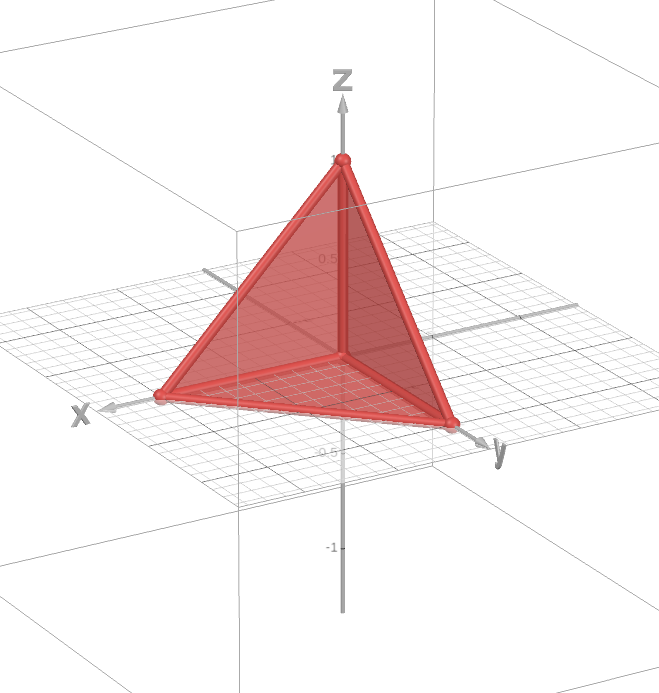
\includegraphics[scale=0.23]{tetrahedron.png}
	\end{center}
	Let's denote the sides in the $XZ$ plane by $S_1$, in the $YZ$ plane by $S_2$, in the $XY$ plane by $S_3$, and the side not in any of the coordinates planes by $S_4$. Therefore, the tetrahedron denoted by $T$ can be decomposed as 
		\[
			T = S_1 \cup S_2 \cup S_3 \cup S_4 .
		\]
	From the statement of the problem, $T$ has the positive orientation (so normal vector is pointing outward). 

	Then, we obtain
		\[
			\iint_T \vec{F} \cdot d\vec{S} = \sum_{j = 1}^4 \iint_{S_j} \vec{F} \cdot \, d\vec{S} .
		\]

	\textbf{\underline{On $S_1$.}}
	A parametrization of $S_1$ is $\vec{r} (x, z) = \left\langle x , 0 , z \right\rangle$, with $0 \leq x \leq 1$ and $0 \leq z \leq 1 - x$. Therefore, $\vec{r}_x \cdot \vec{r}_z = \left\langle 0, -1, 0 \right\rangle$ and hence
		\[
			 \iint_{S_1} \vec{F} \cdot \, d\vec{S} = \iint_D \left\langle 0 , z , x \right\rangle \cdot \left\langle 0, -1, 0 \right\rangle \, dA = -\int_0^1 \int_0^{1 - x} z \, dz dx = -\frac{1}{6} .
		\]

	\textbf{\underline{On $S_2$.}}
	A parametrization of $S_2$ is $\vec{r} (z, y) = \left\langle 0 , y , z \right\rangle$, for $0 \leq z \leq 1$ and $0 \leq y \leq 1 - z$. Therefore, $\vec{r}_z \times \vec{r}_y = \left\langle -1 , 0, 0 \right\rangle$ and hence
		\[
			\iint_{S_2} \vec{F} \cdot d\vec{S} = \iint_D \left\langle y , z - y , 0 \right\rangle \cdot \left\langle -1, 0, 0 \right\rangle \, dA = -\int_0^1 \int_0^{1 - z} y \, dy dz = -\frac{1}{6} . 
		\]

	\textbf{\underline{On $S_3$.}}
	A parametrization of $S_3$ is $\vec{r} (y, x) = \left\langle x, y, 0 \right\rangle$, for $0 \leq y \leq 1$ and $0 \leq x \leq 1 - y$. Therefore, $\vec{r}_y \times \vec{r}_x = \left\langle 0, 0, -1 \right\rangle$ and hence
		\[
			\iint_{S_3} \vec{F} \cdot d \vec{S} = \iint_D \left\langle y, -y , x \right\rangle \cdot \left\langle 0 , 0 , -1 \right\rangle \, dA = -\int_0^1 \int_0^{1 - y} x \, dx dy = -\frac{1}{6} .
		\]

	\textbf{\underline{On $S_4$.}}
	A parametrization of $S_4$ is $\vec{r} (x, y) = \left\langle x, y, 1 - x - y \right\rangle$, for $0 \leq x \leq 1$ and $0 \leq y \leq 1 - x$. We then have
		\[
			\vec{r}_x = \left\langle 1, 0, -1 \right\rangle \quad \text{ and } \quad \vec{r}_y = \left\langle 0, 1, -1 \right\rangle 
		\]
	so that
		\[
			\vec{r}_x \times \vec{r}_y = \left\langle 1, 1, 1 \right\rangle .
		\]
	Hence,
		\[
			\iint_{S_4} \vec{F} \cdot d \vec{S} = \iint_D \left\langle y , 1 - x - 2y , x \right\rangle \cdot \left\langle 1, 1, 1 \right\rangle \, dA = \int_0^1 \int_0^{1 - x} (1 - y) \, dy dx = \frac{1}{3} 
		\]

	\textbf{\underline{Final Answer.}}
	Summing up, we obtain
		\[
			\iint_T \vec{F} \cdot d \vec{S} = -\frac{3}{6} + \frac{1}{3} = \fbox{$-\displaystyle\frac{1}{6}$} \,\,.
		\]



	On the next page, there is a picture of the vectors $\vec{r}_u \times \vec{r}_v$ for each faces of the tetrahedron. Copy-paste \url{https://www.desmos.com/3d/fc7631c3a2} in an internet browser to access the Desmos app and see the tetrahedron live).
		\begin{center}
		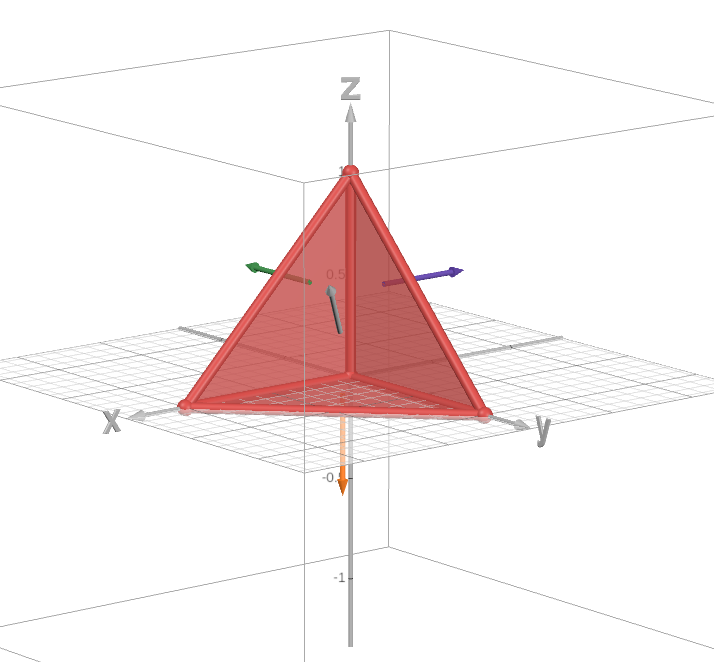
\includegraphics[scale=0.4]{NormalsTetrahedron.png}
		\end{center}



	\spc 

\end{document}